
% \tikzset{every picture/.style={line width=0.75pt}} %set default line width to 0.75pt        

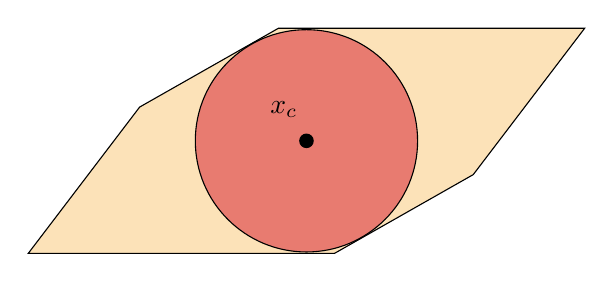
\begin{tikzpicture}[x=0.75pt,y=0.75pt,yscale=-0.7,xscale=0.7]
%uncomment if require: \path (0,300); %set diagram left start at 0, and has height of 300

%Snip Diagonal Corner Rect [id:dp285744847982357] 
\draw  [fill={rgb, 255:red, 245; green, 166; blue, 35 }  ,fill opacity=0.32 ] (286.75,53) -- (497.5,53) -- (497.5,53) -- (420.8,153.75) -- (325.25,208) -- (114.5,208) -- (114.5,208) -- (191.2,107.25) -- cycle ;
%Shape: Circle [id:dp4209627583449631] 
\draw  [fill={rgb, 255:red, 208; green, 2; blue, 27 }  ,fill opacity=0.46 ] (229.5,130.5) .. controls (229.5,88.25) and (263.75,54) .. (306,54) .. controls (348.25,54) and (382.5,88.25) .. (382.5,130.5) .. controls (382.5,172.75) and (348.25,207) .. (306,207) .. controls (263.75,207) and (229.5,172.75) .. (229.5,130.5) -- cycle ;
%Shape: Circle [id:dp17296463065051126] 
\draw  [fill={rgb, 255:red, 0; green, 0; blue, 0 }  ,fill opacity=1 ] (301.38,130.5) .. controls (301.38,127.95) and (303.45,125.88) .. (306,125.88) .. controls (308.55,125.88) and (310.63,127.95) .. (310.63,130.5) .. controls (310.63,133.05) and (308.55,135.13) .. (306,135.13) .. controls (303.45,135.13) and (301.38,133.05) .. (301.38,130.5) -- cycle ;

% Text Node
\draw (279.33,101.67) node [anchor=north west][inner sep=0.75pt]   [align=left] {$\displaystyle x_{c}$};


\end{tikzpicture}